\documentclass[border=10pt]{standalone}
\usepackage{amsmath,amssymb}
\usepackage{tikz}
\usetikzlibrary{shapes.geometric, arrows.meta, positioning, calc, fit, backgrounds}

\begin{document}
\begin{tikzpicture}[
    font=\sffamily,
    >=Stealth,
    node distance=1.4cm and 1.6cm,
    block/.style={draw=blue!70!black, fill=blue!8, line width=1.2pt, rounded corners=4pt, text centered, inner sep=6pt},
    fileblock/.style={draw=green!60!black, fill=green!8, line width=1.2pt, text centered, inner sep=5pt},
    simblock/.style={draw=purple!70!black, fill=purple!8, line width=1.2pt, rounded corners=4pt, text centered, inner sep=6pt},
    passblock/.style={draw=green!60!black, fill=green!15, line width=1.4pt, rounded corners=6pt, text centered, inner sep=8pt},
    bus/.style={line width=1.3pt, ->}
]

    % Software Domain
    \node[block, minimum width=4.5cm] (py_model) {
        \textbf{Python Float32 Reference}\\
        \textbf{\texttt{winograd.py} / \texttt{direct\_conv.py}}\\
        \footnotesize Standard Winograd algorithm
    };

    \node[block, minimum width=4.5cm, below=1.0cm of py_model] (fixed_model) {
        \textbf{INT16 Fixed-Point Model}\\
        \textbf{\texttt{fixed\_point.py}}\\
        \footnotesize Emulates bit-growth, shifts, saturation
    };

    \node[block, minimum width=4.5cm, below=1.0cm of fixed_model] (gen_vec) {
        \textbf{Test Vector Generator}\\
        \textbf{\texttt{generate\_vectors.py}}\\
        \footnotesize Randomized matrices \& stimuli
    };

    % Files Exported
    \node[fileblock, right=1.6cm of fixed_model, yshift=0.8cm] (hex_in) {\textbf{\texttt{input.hex}}};
    \node[fileblock, right=1.6cm of fixed_model, yshift=-0.0cm] (hex_w) {\textbf{\texttt{weight.hex}}};
    \node[fileblock, right=1.6cm of fixed_model, yshift=-0.8cm] (hex_exp) {\textbf{\texttt{expected\_output.hex}}};

    % RTL Simulation Domain
    \node[simblock, minimum width=4.8cm, right=1.6cm of hex_w] (tb) {
        \textbf{Self-Checking SystemVerilog TB}\\
        \textbf{\texttt{winograd\_core\_tb.sv}}\\
        \footnotesize File I/O, Handshake sequencing
    };

    \node[simblock, minimum width=4.8cm, below=1.0cm of tb] (rtl_dut) {
        \textbf{Device Under Test (DUT)}\\
        \textbf{\texttt{winograd\_top.sv}}\\
        \footnotesize Pipelined RTL Datapath + FSM
    };

    % Assertion & Status
    \node[passblock, draw=green!60!black, fill=green!15, minimum width=5.0cm, right=1.6cm of tb] (checker) {
        \textbf{Bit-Exact Assertion Checker}\\
        \vspace{0.1cm}
        \small Compare \texttt{y\_tile} vs \texttt{expected\_output}\\
        \small Automated mismatch counter\\
        \vspace{0.15cm}
        \large\textbf{\color{green!50!black}[PASSED] 0 Mismatches}
    };

    % Connections
    \draw[bus] (py_model) -- node[right, font=\footnotesize] {Cross-validation} (fixed_model);
    \draw[bus] (fixed_model) -- (gen_vec);
    \draw[bus] (gen_vec.east) -- ++(0.5,0) |- (hex_in.west);
    \draw[bus] (gen_vec.east) -- (hex_w.west);
    \draw[bus] (gen_vec.east) -- ++(0.5,0) |- (hex_exp.west);

    \draw[bus] (hex_in.east) -- (tb.170);
    \draw[bus] (hex_w.east) -- (tb.190);
    \draw[bus] (hex_exp.east) -- ++(0.6,0) |- (checker.west);

    \draw[bus] (tb.south) -- node[right, font=\footnotesize] {Stimulus (\texttt{d\_tile}, \texttt{u\_tile})} (rtl_dut.north);
    \draw[bus] (rtl_dut.east) -| node[pos=0.3, right, font=\footnotesize] {Hardware Output (\texttt{y\_tile})} (checker.south);
    \draw[bus] (tb.east) -- node[above, font=\footnotesize] {\texttt{exp\_data}} (checker.west);

    % Background Groups
    \begin{scope}[on background layer]
        \node[draw=blue!40, fill=blue!2, dashed, line width=1.2pt, rounded corners=6pt,
              fit=(py_model) (gen_vec),
              inner sep=8pt,
              label={[font=\bfseries\color{blue!80!black}, anchor=north]north:Software Golden Modeling}] {};

        \node[draw=purple!40, fill=purple!2, dashed, line width=1.2pt, rounded corners=6pt,
              fit=(tb) (rtl_dut) (checker),
              inner sep=8pt,
              label={[font=\bfseries\color{purple!80!black}, anchor=north]north:Automated Hardware Simulation}] {};
    \end{scope}

\end{tikzpicture}
\end{document}
